\section{Thiết kế hệ thống}
\subsection{Hệ thống xử lý câu truy vấn SQL}
\hspace*{1cm} Để có thể xử lý câu truy vấn được nhập từ User. Nghiên cứu các giải pháp sao cho có thể nhận câu SQL người chơi đã nhập, xử lý và trả kết quả về cho hệ thống xử lý và đưa ra các phản ứng của game. Có rất nhiều hướng tiếp cập khác nhau. Nhưng nhóm cũng lựa chọn một số hướng tiếp cận nhất định.
\subsubsection{Hướng tiếp cận sử dụng SQL Server tại Localhost}
\hspace*{1cm} Hướng tiếp cận này sử dụng module SQL và DB là một process độc lập và việc giao tiếp giữa DB và Game là thông qua việc kết nối Database thông qua địa chỉ Localhost và một port nhất định. Việc thiết lập SQL Database Server là riêng biệt. Về phía Game Client chỉ gần thiết lập một connector, sử dụng làm client rồi kết nối đến process Server Local. Các câu truy vấn và dữ liệu trả về sẽ được giao tiếp thông qua connector này.
\begin{figure}[H]
	\centering
	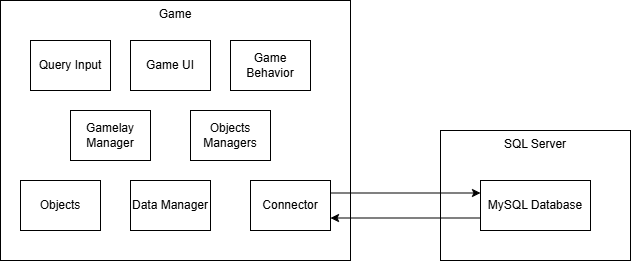
\includegraphics[width=\textwidth]{Images/SQLLocalServer.png}
	\vspace{0.5cm}
	\caption{Mô hình cấu trúc của hướng giải pháp chạy SQL Server trên Local}
\end{figure}
Dưới đây là đoạn code mẫu cho việc kết nối đến SQL Server và gọi yêu cầu thực thi truy vấn từ client\\
\begin{verbatim}
	using System;
	using MySql.Data.MySqlClient;
	
	public class DatabaseConnection
	{
		private MySqlConnection connection;
		
		public void Initialize()
		{
			string connectionString = "Server=localhost;Database=yourdatabase;Uid=yourusername;Pwd=yourpassword;";
			connection = new MySqlConnection(connectionString);
		}
		
		public void OpenConnection()
		{
			try
			{
				connection.Open();
				Console.WriteLine("Connection opened successfully.");
			}
			catch (Exception ex)
			{
				Console.WriteLine("An error occurred: " + ex.Message);
			}
		}
		
		public void CloseConnection()
		{
			try
			{
				connection.Close();
				Console.WriteLine("Connection closed successfully.");
			}
			catch (Exception ex)
			{
				Console.WriteLine("An error occurred: " + ex.Message);
			}
		}
		
		public void ExecuteQuery(string query)
		{
			try
			{
				OpenConnection();
				MySqlCommand cmd = new MySqlCommand(query, connection);
				cmd.ExecuteNonQuery();
				Console.WriteLine("Query executed successfully.");
			}
			catch (Exception ex)
			{
				Console.WriteLine("An error occurred: " + ex.Message);
			}
			finally
			{
				CloseConnection();
			}
		}
	}
\end{verbatim}
\hspace*{1cm} Với việc sử dụng một process riêng, ta có thể tuỳ biến process theo dạng Hệ cơ sở dữ liệu SQL nào đều được, bao gồm MySQL, PostgreSQL,... Miễn là ta lựa chọn thư viện Database Client cho Connector phù hợp là được. Ta sẽ có toàn bộ chức năng như một hệ cơ sở dữ liệu thuần tuý, ta có thể thiết lập các stored procedure, function, thiết lập các quyền cho các user khác nhau cũng như nhiều tính năng hỗ trợ hơn.\\
\hspace*{1cm} Tuy nhiên, với việc sử dụng một process riêng và có sử dụng port. Nếu không xử lý port hợp lý, port mà process chiếm dụng sẽ không được sử dụng cho mục đích khác nữa. Hơn nữa, việc chạy localhost server bản chất vẫn là process, và nó có thể chấm dứt bởi trình quản lý tác vụ của hệ điều hành. Nếu mất đi kết nối với server local, game sẽ không thể thực thi các tác vụ có liên quan đến SQL, game sẽ không thể hoạt động và đó là điều không thể chấp nhận được. Hơn nữa, việc khởi chạy game đòi hỏi game cũng phải khởi chạy thêm tiến trình server. Cũng như khi cài đặt trò chơi, ta phải cài đặt thêm SQL Server. Khiến cho cấu trúc lủng củng, không nhất quán, đặc biệt là nếu SQL Server có sự cố thì game cũng không hoạt động được, dẫn đến chạy không ổn định.
\subsubsection{Hướng tiếp cận xây dựng Hệ cơ sở dữ liệu SQLite ngay trong game}
\hspace*{1cm} Thay vì sử dụng một process riêng biệt, hướng tiếp cận này sử dụng SQLite, là một hệ cơ sở dữ liệu gọn nhẹ, có khả năng nhúng vào các ứng dụng khác. Đây là một ưu điểm lớn của SQLite khi nó có thể thực hiện các câu truy vấn ngay trong lòng ứng dụng, giúp cho cấu trúc được nhất quán và hoạt động đồng nhất và ổn định.
\begin{figure}[H]
	\centering
	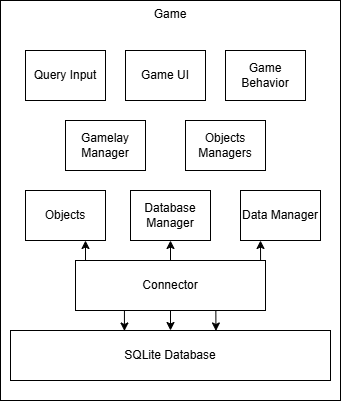
\includegraphics[width=\textwidth]{Images/SQLITE.png}
	\vspace{0.5cm}
	\caption{Cấu trúc game với Hệ cơ sở dữ liệu SQLite}
\end{figure}
\hspace{1cm} Cách thiết lập cũng khá đơn giản, chỉ cần một file .db, cùng với các dependencies cho SQLite hoạt động, và một module connector để kết nối với cơ sở dữ liệu cục bộ, connector cũng đóng vai trò thực hiện các câu truy vấn từ hệ thống và người chơi. Dưới đây là hai đoạn code cho Database Management va Execution cho việc kết nối database cục bộ dạng file và thực thi câu truy vấn. Đoạn code sử dụng SQliter, một công cụ hỗ trợ xử lý kết nối đễn database cục bộ.
\begin{verbatim}
	using System;
	using System.Collections;
	using System.Collections.Generic;
	using UnityEngine;
	using System.Data;
	using Mono.Data.SqliteClient;
	using System.IO;
	using System.Linq;
	using System.Text;
	using SQLiter;
	using Unity.VisualScripting.Dependencies.Sqlite;
	
	namespace Backend
	{
		public class DatabaseManagement : MonoBehaviour
		{
			public bool DebugMode = true;
			
			//public object BackendService;
			
			
			private string sqlDBLocation;
			
			
			//private const string SQL_DB_NAME = "AnimalFantasy";
			
			
			/// <summary>
			/// DB objects
			/// </summary>
			private IDbConnection connection = null;
			private IDbCommand command = null;
			private IDataReader reader = null;
			
			public IDbConnection DBConnection => new SqliteConnection(sqlDBLocation);
			public IDbCommand DBCommand => command;
			public IDataReader DBReader => reader;
			
			//private string sqlString;
			
			//public bool createNewTable = true;
			
			/// <summary>
			/// Awake will initialize the connection.  
			/// RunAsyncInit is just for show.  You can do the normal SQLiteInit to ensure that it is
			/// initialized during the AWake() phase and everything is ready during the Start() phase
			/// </summary>
			private void Awake()
			{
				//if (DebugMode)
				//	Debug.Log("--- Awake ---");
				
				// here is where we set the file location
				// ------------ IMPORTANT ---------
				// - during builds, this is located in the project root - same level as Assets/Library/obj/ProjectSettings.
				// - during runtime (Windows at least), this is located in the SAME directory as the executable.
				// you can play around with the path if you like, but build-vs-run locations need to be taken into account.
				sqlDBLocation = "URI=file:" + DBConfiguation.SQL_PATH + DBConfiguation.SQL_DB_NAME + ".db";
				
				//Debug.Log(_sqlDBLocation);
				
				//Instance = this;
				SQLiteInitialize();
				GlobalContainer.GetGameContainer.Register<DatabaseManagement>(this);
			}
			
			
			
			
			/// <summary>
			/// Clean up SQLite Connections, anything else.
			/// </summary>
			private void OnDestroy()
			{
				SQLiteClose();
			}
			
			/// <summary>
			/// Example using the Loom to run an asynchronous method on another thread so SQLite lookups.
			/// do not block the main Unity thread.
			/// </summary>
			public void RunAsyncInit()
			{
				LoomManager.Loom.QueueOnMainThread(() =>
				{
					SQLiteInitialize();
				});
			}
			
			private void SQLiteClose()
			{
				if (reader != null && !reader.IsClosed)
				reader.Close();
				reader = null;
				
				if (command != null)
				command.Dispose();
				command = null;
				
				if (connection != null && connection.State != ConnectionState.Closed)
				connection.Close();
				connection = null;
				Events.OnDBClosed.Invoke();
			}
\end{verbatim}

\begin{verbatim}
	using System;
	using System.Collections;
	using System.Collections.Generic;
	using UnityEngine;
	using System.Data;
	using Mono.Data.SqliteClient;
	using System.IO;
	using System.Linq;
	using System.Text;
	using JetBrains.Annotations;
	using SQLiter;
	using Unity.VisualScripting.Dependencies.Sqlite;
	/// <summary>
	/// Backend will be responsible for Initialize the Database, using SQL Schema as a playground where player will use SQL Language to interact with game.
	/// UserExecution will be used for processing SQL Command typed by Player, include attack() and use() procedure
	/// BackendExecution will be used for processing SQL Command demanded by the Object Manager. This will have more permission than UserExecution.
	/// Initializer (SQLInitializer) is used for Initializing the game state (include SQL State Initialize) - use to load game, level or progress.
	/// </summary>
	namespace Backend
	{
		
		public class QueryResponse
		{
			public string query;
			public bool Success;
			[CanBeNull] public List<Dictionary<string, object>> results = null;
			[CanBeNull] public Exception error = null;
		}
		
		public class QueryRequest
		{
			public CommandType CType;
			public string tableName;
			[CanBeNull] public Dictionary<string, object> data = null;
		}
		
		
		public class Execution : MonoBehaviour
		{
			
			public bool DebugMode = false;
			
			
			
			/// <summary>
			/// DB objects
			/// </summary>
			private IDbConnection _connection = null;
			private IDbCommand _command = null;
			private IDataReader _reader = null;
			
			public bool _createNewTable = true;
			
			/// <summary>
			/// Awake will initialize the connection.  
			/// RunAsyncInit is just for show.  You can do the normal SQLiteInit to ensure that it is
			/// initialized during the AWake() phase and everything is ready during the Start() phase
			/// </summary>
			void Awake()
			{
				
			
				
				GlobalContainer.GetGameContainer.Register<Execution>(this);
				
				_connection = GlobalContainer.GetGameContainer.Resolve<DatabaseManagement>().DBConnection;
				_command = _connection.CreateCommand();
			}
			
			/// <summary>
			/// Unity Start
			/// </summary>
			void Start()
			{
				
				
				// just for testing, comment/uncomment to play with it
				// note that it MUST be invoked after SQLite has initialized, 2-3 seconds later usually.  1 second is cutting it too close
			}
			
			
			
			
			/// <summary>
			/// Uncomment if you want to see the time it takes to do things
			/// </summary>
			//void Update()
			//{
				//    Debug.Log(Time.time);
				//}
			
			/// <summary>
			/// Clean up SQLite Connections, anything else
			/// </summary>
			void OnDestroy()
			{
				SQLiteClose();
			}
			
			/// <summary>
			/// Basic execute command - open, create command, execute, close
			/// </summary>
			/// <param name="commandText"></param>
			public void ExecuteNonQuery(string commandText)
			{
				_connection.Open();
				_command.CommandText = commandText;
				_command.ExecuteNonQuery();
				_connection.Close();
			}
			
			/// <summary>
			/// Clean up everything for SQLite
			/// </summary>
			private void SQLiteClose()
			{
				if (_reader != null && !_reader.IsClosed)
				_reader.Close();
				_reader = null;
				
				if (_command != null)
				_command.Dispose();
				_command = null;
				
				if (_connection != null && _connection.State != ConnectionState.Closed)
				_connection.Close();
				_connection = null;
			}
			
			public QueryResponse ExecuteQuery(string commandText)
			{
				QueryResponse result = new QueryResponse();
				try
				{
					_connection.Open();
					
					// if you have a bunch of stuff, this is going to be inefficient and a pain.  it's just for testing/show
					_command.CommandText = commandText;
					_reader = _command.ExecuteReader();
					//if (_reader.)
					
					var _header = new List<string>();
					//Debug.Log(_header);
					DataTable dt = _reader.GetSchemaTable();
					foreach (DataRow row in dt.Rows)
					{
						_header.Add(row.Field<string>("ColumnName"));
					}
					List<List<string>> rows = new List<List<string>>();
					while (_reader.Read())
					{
						// reuse same stringbuilder
						List<string> rowValue = new List<string>();
						
						for (int i = 0; i < _header.Count; i++)
						{
							rowValue.Add(_reader.GetString(i));
						}
						/*
						sb.Length = 0;
						
						sb.Append(_reader.GetString(0)).Append(" ");
						sb.Append(_reader.GetString(1)).Append(" ");
						
						sb.AppendLine();
						*/
						
						// view our output
						if (DebugMode)
						//Debug.Log(sb.ToString());
						rowValue.ToString();
						rows.Add(rowValue);
						
					}
					_reader.Close();
					_connection.Close();
					rows.Insert(0, _header);
					Events.OnSelectDisplay.Invoke(rows);
				}
				catch (Exception e)
				{
					result.Success = false;
					result.error = e;
					_reader.Close();
					_connection.Close();
					//Events.OnErrorDisplay.Invoke(e);
					//throw;
				}
				
				
				return result;
			}
		}
	}
	
\end{verbatim}
\hspace*{1cm} Tuy nó có sự tiện lơi và gọn nhẹ và dễ dàng nhúng vào các ứng dụng khác, nhưng đổi lại, nó phải hy sinh nhiều tính năng. Nó không hỗ trợ cấp quyền cho người dùng, nên việc xử lý trên schema sẽ phải thêm một số bước mới có thể cho kỳ vọng. Ngoài ra, với việc không có stored procedure cũng là một thiệt thòi lớn cho những ai muốn sử dụng procedure.\\
\hspace*{1cm} Bỏ qua những khuyết điẻm mà giải pháp này còn tồn đọng, nhóm vẫn quyết định sử dụng giải pháp này vì tính nhất quán và đồng nhất với dự án. Các vấn đề phát sinh nhóm sẽ có những cách xử lý khác nhau.
\subsection{Schema chính của game}
\hspace*{1cm} Một trong những thứ không thể thiếu của game là schema của trò chơi. Người chơi sẽ sử dụng các câu truy vấn SQL để khai thác tối đa SQL, tìm được mục tiêu và tiêu diệt chúng.
\begin{figure}[H]
	\centering
	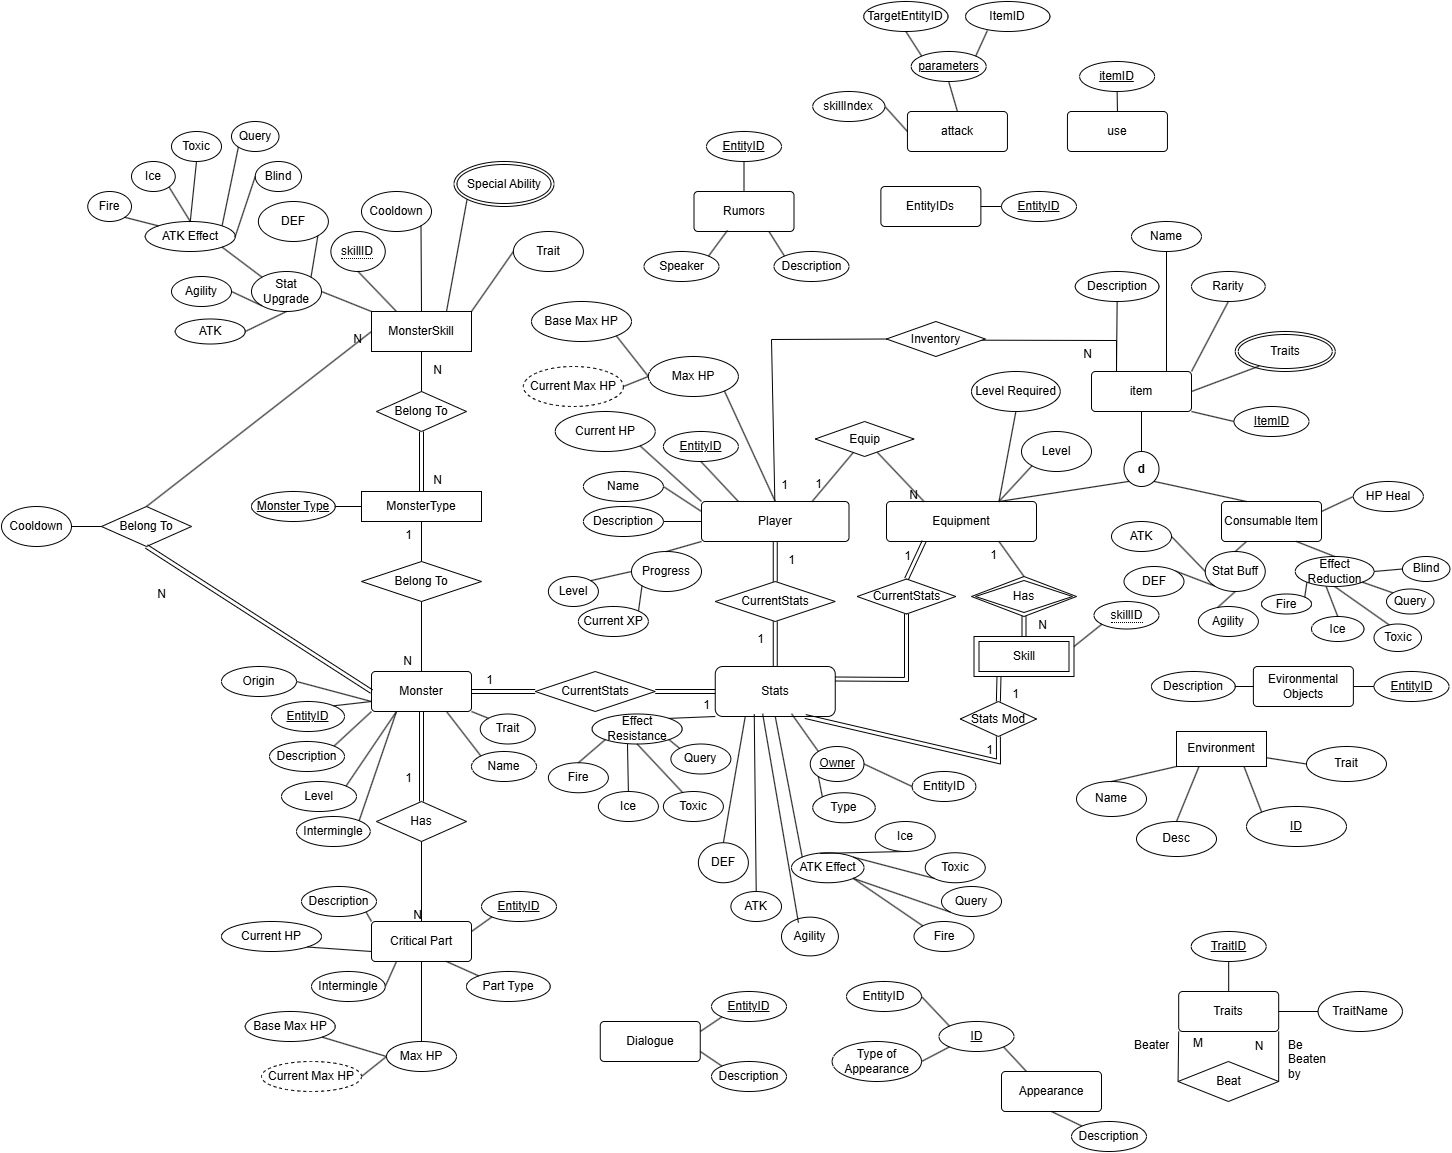
\includegraphics[width=\textwidth]{Images/SchemaEERD.png}
	\vspace{0.5cm}
	\caption{Schema EERD của game}
\end{figure}
\subsection{Xử lý các hành vi ngoại lệ của người chơi}

\hspace*{1cm} Trong quá trình chơi, khó mà tránh khỏi việc người chơi có những hành vi cố ý tác động đến schema, nếu không xử lý hợp lý sẽ gây tình trạng màn chơi bị rối loạn, cũng như có thể dẫn đến mất ổn định game. Luôn nhớ rằng Schema chỉ là Playground của game, các object của game chỉ được quản lý bởi hệ thống, nên việc xử lý phải mang tính răn đe, cho người chơi nhớ được mọi hành vi của bản thân đều có thể mang lại hậu quả, tương tự với việc xử lý SQL trong công việc thực tế.

\hspace*{1cm} Với việc nhóm quyết định sử dụng SQLite và tích hợp thẳng vào game. Khiến nó bộc lộ hạn chế lớn: nó không hỗ trợ việc phân quyền. Vì vậy nhóm quyết định đặt ra các bộ quy tắc để xử lý ở mức DB Manager khi người chơi có các hành vi sau:

\subsubsection{Chèn (Insert) dữ liệu vào các bảng}
Việc insert dữ liệu vào bảng có thể dẫn đến các hành vi phản hồi của game khác nhau:

\paragraph{Chèn vào các bảng Item, Skills}
Các Item cũng như record đã được quản lý bởi game, nên cho dù người chơi có chèn vào bao nhiêu record dữ liệu giả rồi sử dụng chúng trong hàm attack hoặc use đều vô hiệu. Schema tìm được ID trong quá trình xử lý câu lệnh nhưng đưa vào hệ thống game để thao tác mà không tìm ID cũng vô nghĩa, hệ thống sẽ thông báo đã không có gì xảy ra và lượt thao tác của người chơi kết thúc. Không như việc ID không đúng thì người chơi vẫn có cơ hội nhập lại, việc thêm ID giả vào sẽ mang lại hậu quả nghiêm trọng hơn cho người chơi.

\paragraph{Chèn vào các bảng Monster, Critical Parts}
Ngoại trừ việc chèn vào bảng để giải quyết các quái vật khó nhằn, việc chèn vào bảng các record ``rác'' là hành vi gây bất lợi cho người chơi. Vì số lượng record trong bảng lớn khiến người chơi khó xác định được record đúng (tương tự việc bộ phận quái vật tự tạo các record để ngụy trang).

\paragraph{Chèn dữ liệu vào Environment Objects}
Việc thêm dữ liệu vào Environment Objects là vô nghĩa, không mang lại lợi ích cho người chơi, mà chỉ khiến cho bảng dữ liệu to ra, gây khó khăn cho người chơi trong việc xác định entity id phù hợp.

\paragraph{Chèn record vào bảng Player}
Việc insert record của bảng player là vô nghĩa, vì sau khi insert, game sẽ update lại giá trị của player, nó bao gồm việc loại bỏ các record ``rác'' không được quản lý bởi hệ thống, việc insert là vô nghĩa.

\subsubsection{Cập nhật (Update) record của các bảng}

\paragraph{Cập nhật record của các bảng Item, Skills}
Tương tự với Insert, các Item cũng như record đã được quản lý bởi game. Cho dù người chơi có update vào bao nhiêu record dữ liệu thành theo ý của mình rồi sử dụng chúng trong hàm attack hoặc use đều không có sự thay đổi, game vẫn sẽ lấy giá trị mặc định do game đưa vào schema.

\paragraph{Cập nhật record của các bảng Monster, Critical Parts}
Ngoại trừ việc update để giải quyết các quái vật khó nhằn, việc update các record vào bảng có thể biến record đó trở thành record rác và gây bất lợi cho người chơi. Game manager không chỉ quản lý thông tin record hiện tại mà còn quản lý record trong quá khứ.

\paragraph{Cập nhật record của Environment Objects}
Việc update record của các vật thể trong môi trường có kết quả dẫn đến tương tự với việc delete. Theo gameplay, việc delete record của game object trong môi trường có thể kích hoạt hiệu ứng của vật thể đó, hiệu ứng có thể mang lại lợi thế, bất lợi, thậm chí còn mang hậu quả nghiêm trọng (ví dụ sát thương cho người chơi quá lớn, làm người chơi chết).

\paragraph{Cập nhật record của bảng Player}
Việc update record của bảng player là vô nghĩa, vì sau khi update, game sẽ khôi phục giá trị player về trước khi nó được update.

\subsubsection{Xóa (Delete) dữ liệu khỏi các bảng}

\paragraph{Xóa record các bảng Item, Skills}
Việc xoá record của bảng Item, Skills sẽ mang lại bất lợi cho người chơi. Khi người chơi thực hiện hàm attack, use thì schema sẽ báo lỗi không tìm thấy id phù hợp, khi đó người chơi đến hết màn chơi không thể sử dụng hoặc tấn công bằng item đó nữa.

\paragraph{Xóa record các bảng Monster, Critical Parts}
Ngoại trừ việc xoá record để giải quyết các vấn đề phát sinh từ quái vật khó nhằn, đây là hành vi gây bất lợi cho người chơi. Nếu mất đi record cần thiết, người chơi sẽ không thể xác định được record của bộ phận monster, việc thực thi câu lệnh attack() sẽ trả lỗi ở mức Database.

\paragraph{Xóa dữ liệu Environment Objects}
Tương tự với update record, việc delete record của game object trong môi trường có thể kích hoạt hiệu ứng của vật thể đó, hiệu ứng có thể mang lại lợi thế, bất lợi, thậm chí còn mang hậu quả nghiêm trọng.

\paragraph{Xóa record bảng Player}
Với việc bảng player tự phục hồi, nên việc delete record không có ảnh hưởng gì.


